\chapter[Referencial Teórico]{Referencial Teórico}

Este capítulo apresenta conceitos pertinentes aos principais tópicos abordados nesse TCC. Os tópicos abordados são \textit{Mobile Social Games}, Engenharia de Software e Sistemas MultiAgentes.

\section{Mobile Social Games}
A área de \textit{Mobile Social Games} possui diversos jogos com os mais variados estilos.
Esses estilos podem ser subdivididos em dois grandes grupos: \textit{Hard-Core Games} e \textit{Casual Games}. Ambos possuem características em comum que os definem como \textit{Social Games}, mas também possuem peculiaridades referentes ao tipo de interação social presente no jogo. Os \textit{Hard-Core Games} são caracterizados por serem ambientes de extrema interação social, onde diversas oportunidades para criação de laços de amizade são presentes \cite{cole2007}. \textit{Casual Games} por outro lado, apresentam interações mais casuais em que laços de amizade são mais fracos \cite{ricchetti2015}.

    \subsection{Definição de Mobile Social Games}
Existem diversas definições para \textit{Social Game}, entretanto, todas possuem características semelhantes. De acordo com os autores Bergenti, Caire, Gotta, Park e Lee, \textit{Social Game} é todo o jogo que utiliza uma plataforma, ou serviços, de uma rede social \cite{bergenti2013} \cite{park2012}. Fields define que \textit{Social Game} é um jogo em que as interações entre usuários ajudam na adoção e manutenção de jogadores conectados através de uma rede social externa, facilitando o alcance desses objetivos \cite{fields2014}. Já Matt Ricchetti faz uma definição mais social. Ele define \textit{Social Game} como sendo uma comunidade que possui várias interações presentes em relações sociais, tais como: competição, colaboração, rebelião, inveja e compaixão \cite{ricchetti2015}.

Matt Ricchetti vai além, e também define três características para divisão de \textit{Social Games}. Essas características são baseadas no tipo de interação social e sincronia do jogo \cite{ricchetti2015}. As três características relativas a \textit{Social Games} são:

\begin{itemize}
  \item Interação síncrona vs assíncrona entre usuários. As interações ocorrem simultaneamente em tempo real, ou em tempos diferentes, em um estilo de turnos?;
  \item Formação simétrica vs assimétrica de relações socias. Formar uma relação social requer entrada de dados de ambos os participantes, ou pode ser formada de maneira unilateral?;
  \item Laço forte ou fraco na formação de relações sociais. As relações sociais tendem a ser fortes e duradouras, ou tendem a ser fracas e transitórias?
\end{itemize}

As três definições apresentadas são complementares e utilizadas em conjunto durante esse trabalho.
Por sua vez, \textit{Mobile Social Games} se refere a \textit{Social Games} que são desenvolvidos para plataformas \textit{mobile}, como Android, iOS e Windows Phone.

  \subsection{Perspectiva Histórica de Mobile Social Games}

Os primeiros \textit{Social Games}, assim como os demais jogos de computador, eram bastante simples. Suas interfaces gráficas eram simuladas por texto e a quantidade de opções disponíveis eram limitadas. As primeiras versões de \textit{Social Games} são conhecidas como \textit{Multi-User Dungeons} (MUDs)\cite{edward1997}. Os MUDs possuiam seu estilo de jogo baseado em turnos, mas também permitiam que usuários interagissem de maneira síncrona ou assíncrona, em ambientes com diversas temáticas, desde guerra no espaço, até o velho oeste americano. Os MUDs eram executados em redes sociais conhecidas como \textit{Bulletin Board Systems} (BBS), redes sociais baseadas em sistemas de texto que permitiam a interação entre usuários através de uma rede de telefone \cite{fields2014}. \textit{Trade Wars}, Figura \ref{figura:tradeWars}, é um exemplo de MUD executado em BBS. O \textit{Trade Wars} foi lançado em 1984 e possuia a temática de guerra no espaço. Nele os usuários poderiam competir e formar alianças para conquistar recursos.

\begin{figure}[h]
  \centering
  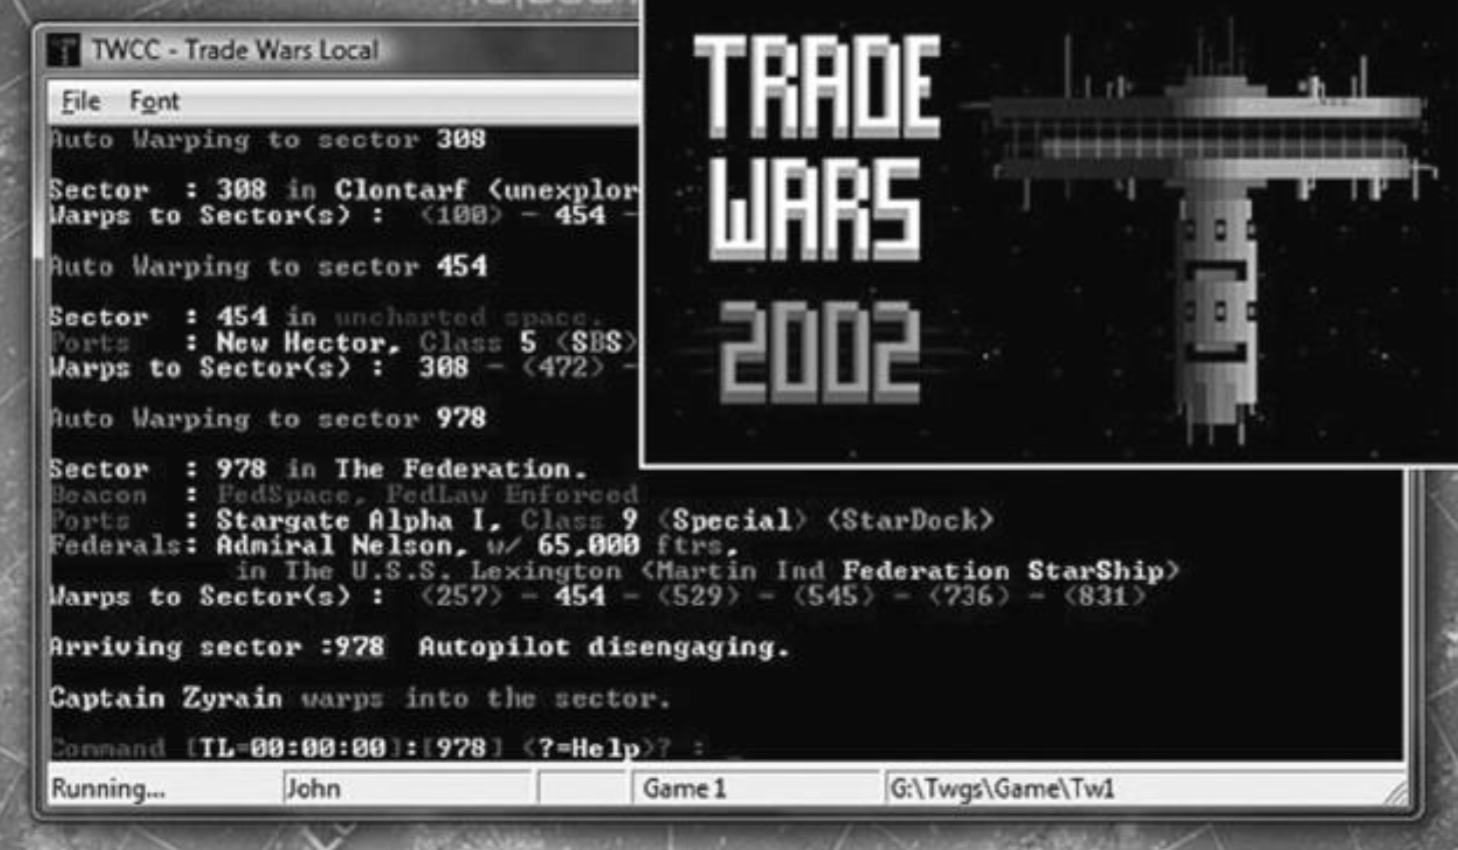
\includegraphics[width=10cm]{figuras/trade_wars.png}
  \caption{MUD \textit{Trade Wars} \cite{fields2014}}
  \label{figura:tradeWars}
\end{figure}

A redução no custo de produção de dispositivos com maior capacidade de processamento, e conexões de internet mais velozes e estáveis, permitiu que interfaces gráficas em nível 2D e 3D, e o acesso aos \textit{Social Games} fosse expandido em diversas plataformas, como \textit{PC} e \textit{Mobile}.

A evolução dos MUDs levou ao desenvolvimento dos \textit{Massively- Multiplayer Online Role-Playing Games} (MMORPGs). Os MMORPGs possuem inúmeras características que os definem como \textit{Social Games}. Nesse estilo de jogo é possível a troca de mensagens entre usuários através de uma rede interna, e muitas vezes externa, \textit{chat} em tempo real, formação de grupos para cooperação e vários outros estilos de organizações sociais \cite{fields2014}.

Um dos MMORPG de maior sucesso para a plataforma PC é o \textit{World of Warcraft}, Figura \ref{figura:wow}. O \textit{World of Warcraft} foi desenvolvido pela \textit{Blizzard Entertainment} em 2004, e possui até o momento da escrita desse trabalho o título de MMORPG mais rentável da história \cite{thurau2010} \cite{omer2015}. \textit{World of Warcraft} é baseado em um mundo medieval de fantasias, nele os jogadores controlam personagens que podem evoluir de level, desenvolver habilidades, participar de guerras, entre outras inúmeras atividades. As atividades sociais do \textit{World of Warcraft} são constantes no jogo. Jogadores interagem em ações de dança, festas, grupos de \textit{chat} e formação de grupos para tarefas que não são possíveis de maneira individual, como conquista de itens especiais \cite{thurau2010} \cite{nardi2006}.

\begin{figure}[h]
  \centering
  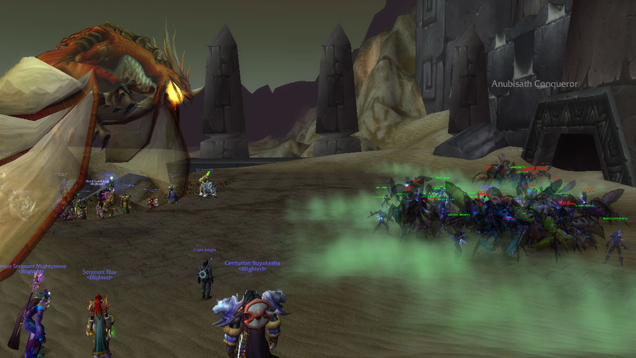
\includegraphics[width=10cm]{figuras/wow.jpg}
  \caption{MMORPG \textit{World of Warcraft} \cite{kotaku}}
  \label{figura:wow}
\end{figure}

Os MMORPG começaram na plataforma \textit{mobile} em 2003 com o lançamento do TibiaME, versão \textit{mobile} do MMORPG Tibia para PC \cite{tibiaME}. O TibiaME é um MMORPG no estilo de fantasia medival em que os jogadores podem evoluir o level dos seus personagens, participar de guerras e grupos sociais. As versões iniciais do TibiaME eram destinadas aos primeiros dispositivos móveis com suporte para J2ME (\textit{Java 2 Platform, Micro Edition}). As primeiras versões possuiam gráficos em 2D, Figura \ref{figura:tibiaME}, devido as restrições de hardware presentes nos primeiros \textit{smartphones}, e necessitavam de acesso constante a internet, sendo essa realizada inicialmente através das primeiras redes 2G.

A evolução do hardware em \textit{smartphones}, novas plataformas, redes móveis mais estáveis e velozes, e paralelamente a criação de novas redes sociais, como o \textit{Facebook}, possibilitou o desenvolvimento e melhoria de inúmeros novos tipos de \textit{Mobile Social Games}, além dos MMORPGs. Alguns desses estilos de \textit{Mobile Social Games} são: \textit{Turn-Based Building Games}, \textit{Simulation Games}, \textit{Virtual Worlds}, \textit{Non-Persistent Action and RTS Games} e \textit{Online Trading Card Games} \cite{fields2014}. Atualmente inúmeros \textit{Mobile Social Games} estão disponíveis em lojas de aplicativos de todas as grandes plataformas, entre elas o Google Play, Apple Store e Windows Phone Store.

\begin{figure}[h]
  \centering
  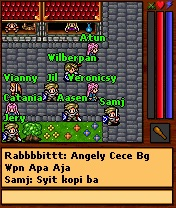
\includegraphics[width=5cm]{figuras/tibiaME}
  \caption{TibiaME. Primeiro MMORPG para plataforma \textit{Mobile} \cite{tibiaMEhistory}}
  \label{figura:tibiaME}
\end{figure}

  \subsection{Problemas Ligados a Mobile Social Games}

Os \textit{smartphones} são dispositivos que estão sempre presente no cotidiano das pessoas. Eles são produzidos por diversas empresas, possuem sistemas operacionais distintos, tamanhos de telas variados, e inúmeras outras especificações de hardware e software diferentes entre si. Essa essência portátil, fragmentação de sistemas operacionais e hardware, rede móvel precária e capacidade de processamento menor que computadores pessoais, são raízes de vários problemas encontrados em \textit{Mobile Social Games}.

De acordo com o \textit{International Data Corporation}, o \textit{marketshare} de sistemas operacionais para \textit{smartphones} é amplamente ocupado pelo Android. No segundo quadrimestre de 2015, o sistema operacional Android possuia 82.8\% do mercado de \textit{smartphones}, enquanto que o segundo maior sistema operacional, Apple iOS, possuia apenas 13.9\% do mercado \cite{idc}. Esses dados poderiam indicar uma maior facilidade para o desenvolvimento de aplicativos para \textit{smartphones}, dado que a maior parte dos dispositivos possui o sistema operacional Android, no entanto essa análise é incorreta. Mesmo possuindo um \textit{marketshare} muito inferior ao Android, o iOS ainda gera uma receita maior que o seu concorrente \cite{appAnnie}. Essa característica faz com que desenvolvedores foquem em ambas as plataformas, visto a oportunidade de geração de receita. Outro problema relacionado ao Android é a sua própria fragmentação. Dados da própria Google demonstram a existência de várias versões do Android, tamanhos de telas e suporte a diferentes versões de \textit{engines} de vídeo \cite{dashboardGoogle}. Todas essas diferenças aumentam os custos e dificultam a criação de \textit{Mobile Social Games} que sejam compatíveis com a maior parte do mercado.

\begin{figure}[h]
  \centering
  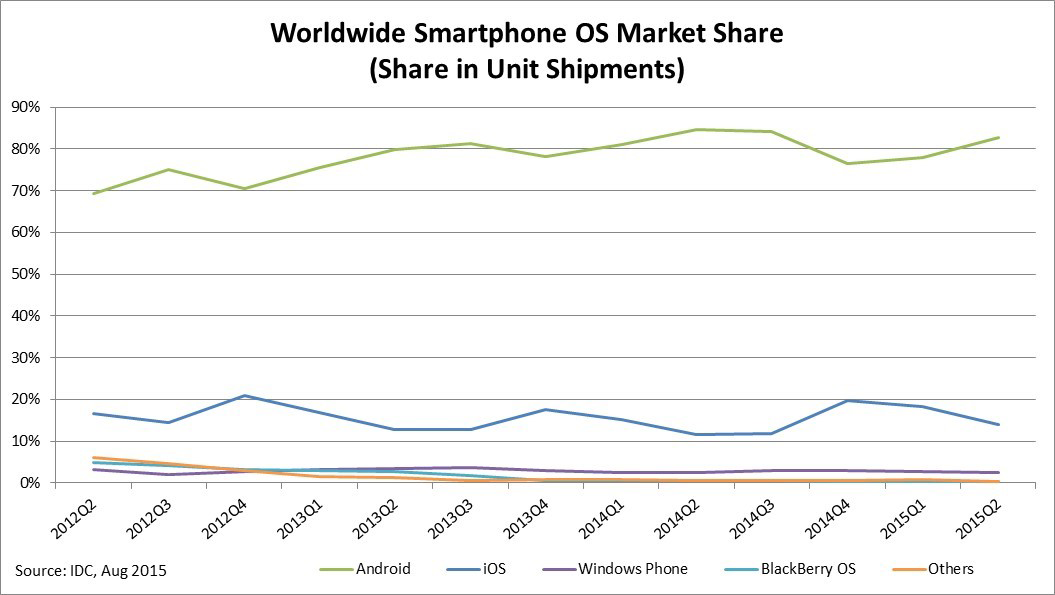
\includegraphics[width=12cm]{figuras/market_share}
  \caption{Quota de mercado de \textit{Smartphones} entre 2012 e 2015 \cite{idc}.}
  \label{figura:market_share}
\end{figure}

\begin{figure}[h]
  \centering
  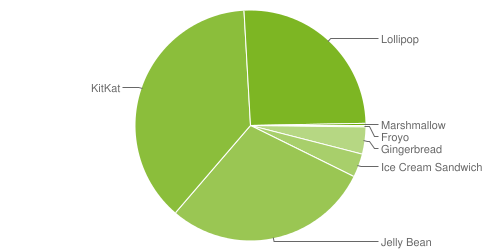
\includegraphics[width=10cm]{figuras/android_chart}
  \caption{Fragmentação das versões do Android em 2015 \cite{dashboardGoogle}.}
  \label{figura:android_chart}
\end{figure}


%Rede/ Latência, velocidade
%Usabilidade(Maybe..)...


  \subsection{Mercado de Mobile Social Games}

\textit{Mobile Games} se tornaram uma das mais importantes plataformas para jogadores e desenvolvedores de jogos. O mercado de \textit{Mobile Games} demonstra crescimento contínuo e números expressivos. Na Figura \ref{figura:gmgcMarket} é possível analisar que em 2014, o mercado de \textit{Mobile Games} apresentou um aumento de receita de 33\% e 55\%, em \textit{smartphones} e \textit{tablets}, respectivamente. Em 2017, a perspectiva é que \textit{Mobile Games} serão responsáveis por 38\% do mercado global de jogos e receita prevista de \$40.4 bilhões de dólares \cite{gmgc}.

\begin{figure}[h]
  \centering
  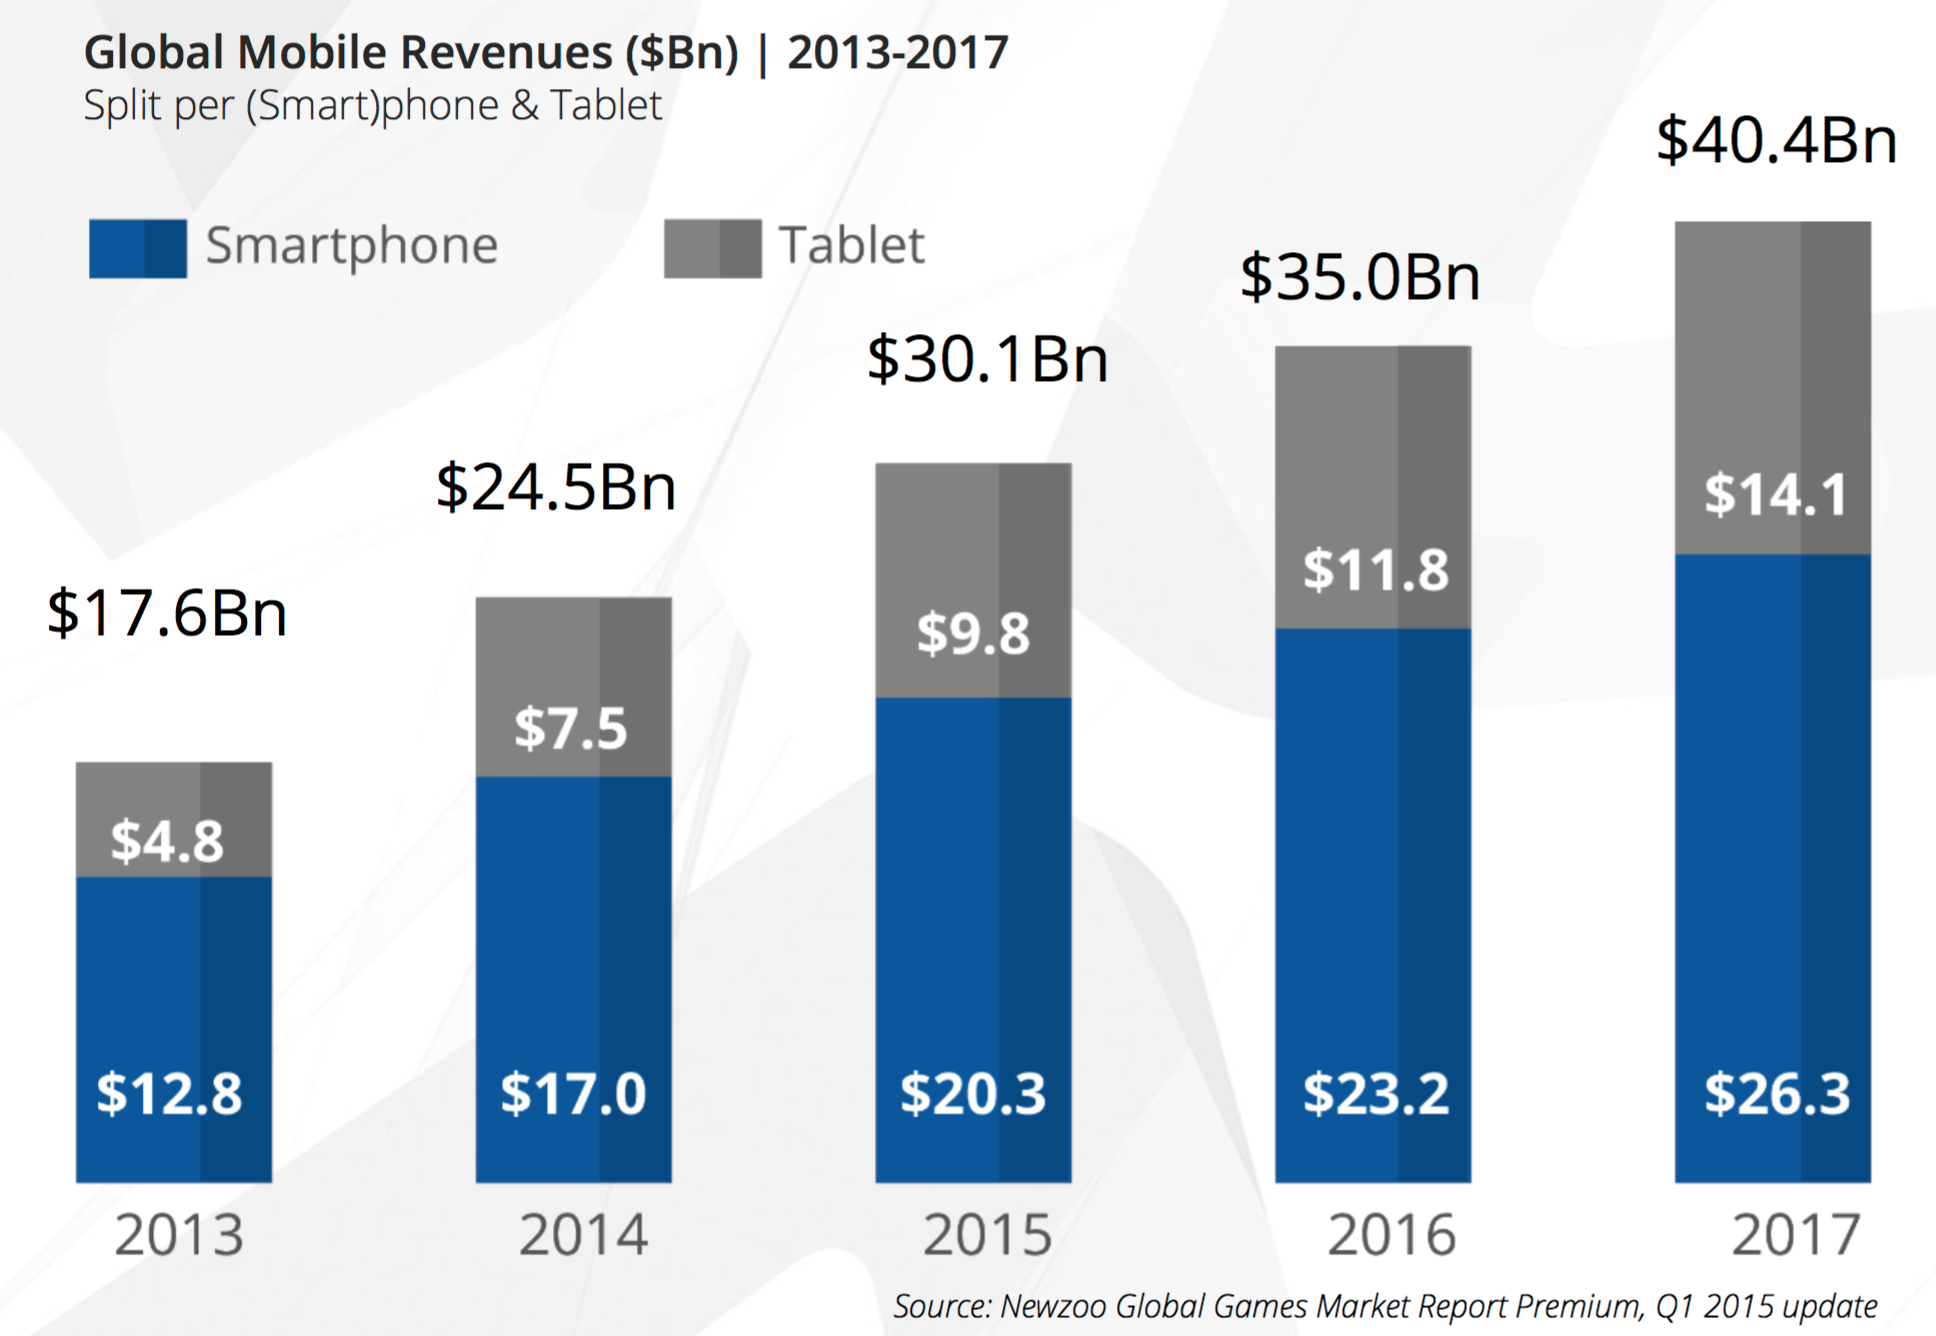
\includegraphics[width=10cm]{figuras/gmgcMarket}
  \caption{Perspectiva de receita para o mercado \textit{Mobile} \cite{gmgc}}
  \label{figura:gmgcMarket}
\end{figure}

O mercado de \textit{Mobile Games} está em constante crescimento e possui características que estão sendo analisadas para o mapeamento dos motivos para o seu sucesso. Fields revela algumas características interessantes do mercado de \textit{Mobile Gaming} nos Estados Unidos da América. Essas características são referentes a distribuição demográfica no ano de 2013 \cite{fields2014}:

\begin{itemize}
  \item As mulheres representam 53\% dos usuários do mercado de \textit{Mobile Games};
  \item 50\% do jogadores possuem entre 25 e 30 anos;
  \item 57\% dos jogadores jogam diariamente, e 54\% jogam por mais de uma hora por dia;
  \item 30\% dos jogadores jogam na cama, e 16\% no ônibus ou metrô.
\end{itemize}

A receita gerada pelo mercado de \textit{Mobile Games} possui números atraentes para os desenvolvedores, no entanto, a monetização de jogos não é uma tarefa fácil. Atrair usuários para o seu jogo em um mercado repleto de opções é uma tarefa difícil, especialmente quando se trata de uma empresa que está iniciando, ou de porte pequeno. Dado essas dificuldades, várias estratégias de monetização de \textit{Mobile Games} são utilizadas \cite{fields2014}:

\begin{itemize}
  \item \textit{Premium download};
  \item \textit{Subscriptions};
  \item \textit{Freemium}.
\end{itemize}

O modelo \textit{Premium download} se caracteriza pela venda completa do jogo para o usuário. O usuário compra o jogo em uma \textit{app store}, como \textit{Google Play} e \textit{Amazon Appstore}, e obtém o jogo em sua completude, sem necessidade a de dispêndios futuros. Esse modelo é normalmente utilizado por estúdios e franquias que já possuem uma grande base de usuários, ou verba suficiente para atrair usuários através de ações publicitárias.
O modelo \textit{Subscriptions} é baseado em assinaturas. O usuário recebe de maneira gratuita os primeiros meses do jogo, sendo necessária uma assinatura posterior para a continuação do jogo. Esse modelo é normalmente utilizado em jogos que necessitam de um grande processamento em \textit{back-end}, como os MMORPG. Esse modelo está em declínio devido ao crescimento de jogos de alta qualidade que utilizam o próximo modelo, o \textit{Freemium}.
O modelo \textit{Freemium} pode ser subdividido em várias categorias, todas com a mesma base: o jogo é gratuito. A monetização com esse modelo é feita através da venda de itens, serviços e propagandas dentro do jogo. Os usuários possuem a possibilidade de comprar itens para aumentar a velocidade de evolução no jogo, liberar áreas indisponíveis e retirar propagandas indesejadas através de pagamento.

Os modelos apresentados podem ser utilizados de maneira singular ou híbrida, o que é necessário, é a análise de qual, ou quais, modelos se adequam ao estilo de jogo implementado, tipo de público alvo, verba disponível para propaganda do jogo, entre outros fatores.

Através dos dados apresentados, fica evidente que o mercado de \textit{Mobile Games} está em um momento de crescimento e geração de inúmeras oportunidades para desenvolvedores independentes e empresas que já estão solidificadas no mercado de jogos. Novas técnicas, princípios, metodologias e paradigmas podem ser a solução para a melhoria do processo de desenvolvimento de \textit{Mobile Social Games}. O próximo capítulo aborda tópicos ligados a Engenharia de Software, como Sistemas MultiAgentes, que podem ser utilizados para abordar alguns dos problemas relatados.

\section{Engenharia de Software}

Dado os objetivos desse trabalho, se dá necessário o embasamento teórico das áreas de Engenharia de Software a serem utilizadas. Dentre elas está a utilização do paradigma MultiAgentes, testes unitários e automatizados para Sistemas MultiAgentes e para a plataforma \textit{mobile} escolhida e técnicas para análise de qualidade de código fonte.

  \subsection{Sistemas MultiAgentes}

A visão baseada em agentes oferece um repertório poderoso de ferramentas, técnicas, e metáforas que possuem um potencial considerável para melhorar a maneira como as pessoas conceitualizão e implementam diferentes tipos de software. Agentes são usados em uma variedade crescente de aplicações — desde sistemas pequenos, como filtros personalizados para emails, até grandes, complexos e críticos sistemas de controle aéreo. À primeira vista, pode parecer que tais sistemas possuem pouco em comum. E no entanto, esse não é o caso: em ambos, a abstração chave utilizada é a de agentes \cite{jennings1998}.

De acordo com Wooldridge, Sistemas MultiAgentes (SMA) são sistemas compostos por múltiplos elementos computacionais que interagem entre si, conhecidos como Agentes. Agentes são sistemas computacionais com duas importantes capacidades. Eles possuem, pelo menos em certo nível, capacidade de agirem de maneira autônoma, de decidirem por si mesmos o que eles precisam fazer para satisfazer os seus objetivos. Eles são capazes de interagir com outros agentes, não simplesmente compartilhando dados,  mas se envolvendo em atividades análogas às atividades sociais em que todos nós nos envolvemos diariamente: cooperação, coordenação, negociação, e similares \cite{wooldridge2009}. As características presentes em um Sistema MultiAgente são  \cite{jennings1998}:

\begin{itemize}
  \item Cada agente possui uma informação incompleta, ou capacidade para resolver um problema, ou seja, cada agente tem uma visão limitada;
  \item Não existe um sistema global de controle;
  \item Os dados são descentralizados e;
  \item Computação é assíncrona.
\end{itemize}

Alguns dos motivos pelo interesse em SMA são: habilidade de prover robustez e eficiência; habilidade para permitir inter-operação entre sistemas legados; e habilidade para resolver problemas em que \textit{data}, \textit{expertise} ou controle são distribuídos \cite{jennings1998}.

    \subsubsection{Tipos de Arquiteturas Orientadas a Agentes}

As arquiteturas de agentes são mecanismos fundamentais, subjacentes aos componentes autônomos, que permitem comportamento efetivo e dinâmico em um mundo real, e em ambientes abertos. As arquiteturas de agentes podem ser divididas em quatro grupos principais: baseados em lógica, reativos, crença-desejo-intenção(\textit{belief, desire, intention}), e em camadas (ou híbrida)\cite{fabio2007}.

A arquitetura \textbf{baseada em lógica} possui sua fundação em técnicas conhecidas de sistemas tradicionais em que o ambiente é representado de forma simbólica e manipulado usando mecanismos de raciocínio\cite{fabio2007}.

Arquiteturas \textbf{reativas} implementam a tomada de decisão como um mapeamento direto da situação para ação, baseando-se em estímulos desencadeados por sensores de dados. Ao contrário da arquitetura \textbf{baseada em lógica}, a arquitetura reativa não possue qualquer modelo simbólico central, e portanto, não utiliza qualquer raciocínio lógico simbólico complexo\cite{fabio2007}.

A arquitetura \textbf{crença-desejo-intenção}, ou BDI (\textit{belief, desire, intention}), é baseada em três estruturas: crença (\textit{belief}), que é o conhecimento que o agente possui do ambiente; desejo (\textit{desire}), que representa os objetivos que ele deve alcançar; e intenção,  que representa as tarefas a serem realizadas pelo agente, ou seja, planos estratégicos visando alcançar os objetivos desejados. (\textit{intention})\cite{fabio2007}.

Por fim, a arquitetura em \textbf{camadas}, ou híbrida, permite tanto o comportamento reativo quanto o deliberativo. Para permitir essa flexibilidade, subsistemas são dispostos como camadas (horizontais e verticais) de maneira hierárquica para acomodar ambos os tipos de agentes \cite{fabio2007}.

  \subsection{Testes de Software}

Teste de Software é um processo, ou uma série de processos, destinado(s) a certificar-se que o código de computador faça o que foi projetado para fazer, e inversamente, não faça algo não planejado\cite{myers2011}.

Myers define os seguintes princípios para o teste de Software\cite{myers2011}:

\begin{itemize}
  \item Testar é o processo de executar o programa com a intenção de encontrar erros;
  \item O teste é mais bem sucedido quando não realizado pelo próprio desenvolvedor;
  \item Um bom caso de teste é aquele que possui uma maior probabilidade de encontrar erros não conhecidos;
  \item Um caso de teste bem sucedido é aquele que detecta um erro desconhecido;
  \item Um teste bem sucedido inclui a definição cuidadosa dos dados de entrada e saída;
  \item Um teste bem sucedido inclui estudar cuidadosamente os resultados obtidos.
\end{itemize}

Teste está presente em todos os estágios do ciclo de desenvolvimento de Software, mas é feito de uma maneira diferente em cada nível. Lu Luo define os seguintes níveis de teste \cite{luo2001}:

\begin{itemize}
  \item \textbf{Teste Unitário:} Teste feito no mais baixo nível. Testa as estruturas unitárias do software, que é a menor parte testável;
  \item \textbf{Teste de Integração:} É realizado quando duas ou mais unidades são combinadas em uma estrutura maior;
  \item \textbf{Teste de Sistema:} Tende a afirmar a qualidade de todo o sistema. Esse teste é muitas vezes baseado em requisitos funcionais do sistema. Atributos de qualidade não funcionais também são verificados;
  \item \textbf{Teste de Aceitação:} É um teste formal destinado a validar a aceitação do sistema diante da avaliação do usuário, cliente ou entidade autorizada.
\end{itemize}

Existem duas categorias de técnicas para teste de software. Diferentes técnicas revelam diferentes aspectos de qualidade do software. As categorias são funcional e estrutural. Os testes funcionais recebem dados de entrada, e sua saída é avaliada para análise da conformidade com o esperado. O teste estrutural também recebe dados de entrada e tem sua saída avaliada, porém a análise vai além, verificando a estrutura interna do sistema ou componente\cite{luo2001}.

O teste funcional, ou caixa-preta, visualiza o sistema como uma caixa-preta. O objetivo não é verificar o comportamento interno ou estrutural, mas sim em quais circunstâncias o programa não se comporta como esperado\cite{myers2011}.

O teste estrutural, ou caixa-branca, permite examinar a estrutura interna do programa. Essa estratégia deriva testes através da lógica do programa. O objetivo é testar todos os caminhos possíveis de execução\cite{myers2011}.

  \subsection{Testes para Dispositivos Android}

A plataforma Android inclui um \textit{framework} integrado que facilita o teste de todos os aspectos dos aplicativos. O SDK (\textit{Software Development Kit}) também fornece ferramentas para a configuração e execução dos testes.

    \subsubsection{O \textit{Framework} de testes}

O \textit{framework} de testes fornece as seguintes características: as \textit{suites} de teste são baseadas no JUnit \cite{junit2015}; as \textit{suites} de testes são contidas em pacotes de teste que são similares aos pacotes da aplicação; o \textit{framework} fornece extensões do JUnit para testes específicos do Android; o SDK pode ser utilizado através da IDE Eclipse ou por comandos de terminal, e o SDK fornece integração com o \textit{monkeyrunner}, uma API para testar dispositivos Android através de código Python.

\begin{figure}[H]
  \centering
  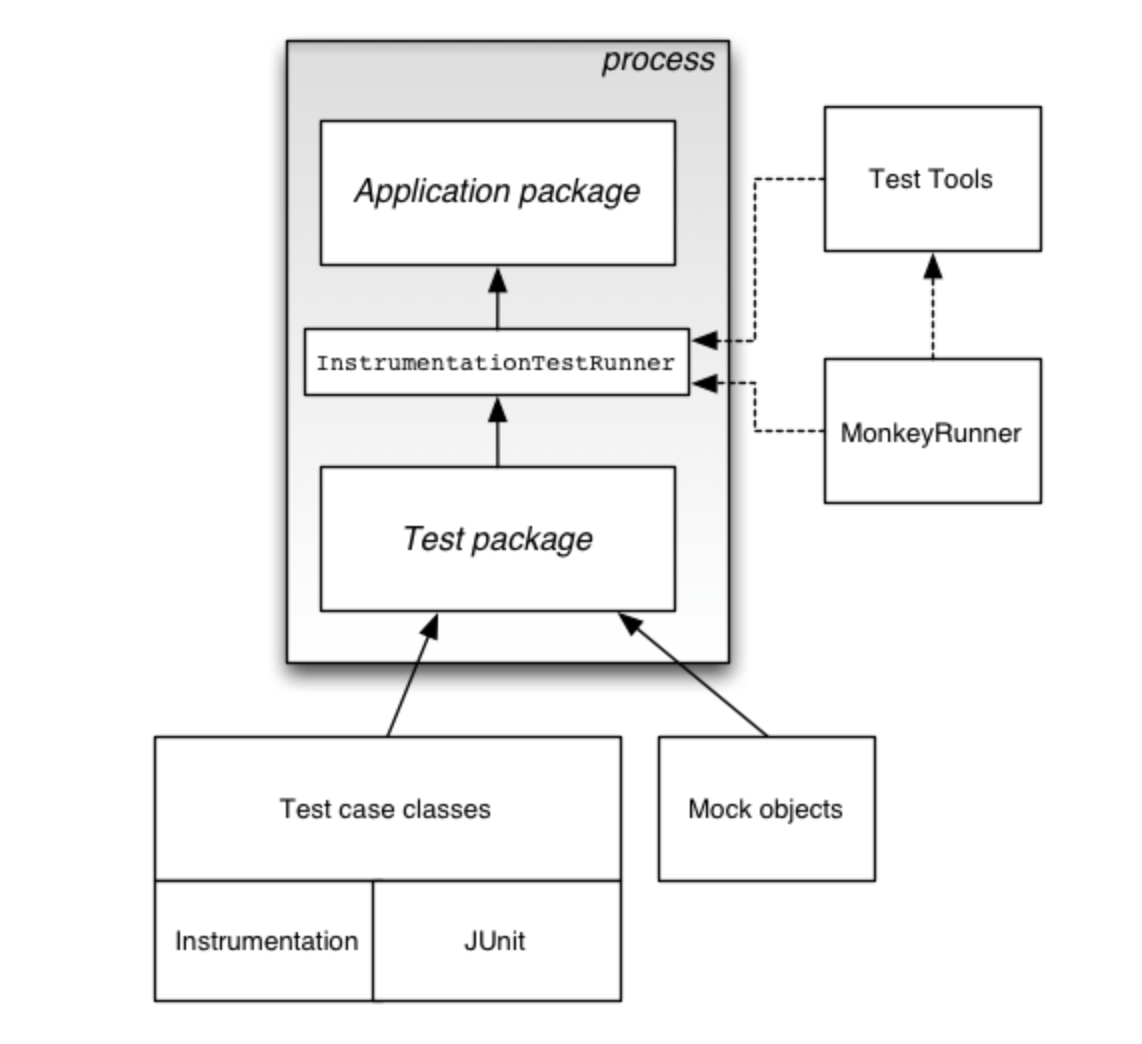
\includegraphics[width=10cm]{figuras/android_test.png}
  \caption{Estrutura do framework de testes \cite{androidTesting2015}}
  \label{figura:testes}
\end{figure}

A Figura \ref{figura:testes} resume a estrutura do \textit{framework} de testes. É possível ver que a estrutura de testes do Android é baseada no JUnit. Portanto, os testes são organizados em classes, pacotes e projeto. O \textit{framework} também disponibiliza um conjunto de métodos, \textit{InstrumentationTestRunner}, que permite a execução de componentes do Android sem as restrições dos ciclos de vida \cite{androidTesting2015}.

O \textit{framework} disponibiliza um conjunto de ferramentas que podem ser utilizadas para diferentes tipos de teste. Como teste de interface gráfica (\textit{Espresso} e \textit{UI Automator}) e testes compatíveis com JUnit3 e JUnit4 (\textit{AndroidJUnitRunner}). Outra ferramenta disponível é o \textit{MonkeyRunner}, uma ferramenta que fornece a opção para criação de testes fora do escopo de código do aplicativo Android.


%  \subsection{Testes para Sistemas MultiAgentes}

%Focar na plataforma JADE
%Discutir sobre o add-on framework
%Well, this is going to take a looooong time

  \subsection{Qualidade de Software}

TODO
%Agents
%Métricas de Qualidade de Código Fonte

\section{Considerações Finais do Capítulo}

TODO
